%%%%%%%%%%%%%%%%%%%%%%%%%%%%%%%%%%%%%%%%%%%%%%%%%%%%%%%%%%%%%%%%
%  EEDURO Delta: Getting Started Guide                         %
%                                                              %
%  Stefan Landis (stefan.landis@ntb.ch)                        %
%  Martin Züger (martin.zueger@ntb.ch)                         %
%%%%%%%%%%%%%%%%%%%%%%%%%%%%%%%%%%%%%%%%%%%%%%%%%%%%%%%%%%%%%%%%

% 1. Definieren der Dokumentklasse.
\documentclass[
  pdftex,                           % PDFTex verwenden um ausschliesslich ein PDF zu erzeugen
  a4paper,                          % A4 Papier
  doubleside,                       % Doppelseitiger Druck
  11pt,                             % Standard Schriftgrösse
  parskip=half,                     % Europäischer Satz mit Abstand zwischen Absätzen
  headsepline,                      % Linie nach Kopfzeile
  ]{scrreprt}                       % KOMA-Script Klasse

% 2. Zeichencodierung und Zeichensatz
\usepackage[utf8]{inputenc}         % 'utf8' -> nicht kompatibel mit TeXnicCenter (unterstützt kein UTF-8)
\usepackage[T1]{fontenc}            % 'T1' Codierung für die Schrift

% 3. Lokalisierung
\usepackage[english, american]{babel}
\usepackage{textcomp}               % Euro Symbol (\texteuro}
\usepackage{upgreek}				% Paket für nichtkursive griechische Kleinbuchstaben

% 4. Schriften
\usepackage{courier}                % Courier laden (wird für Code verwendet)
\usepackage{helvet}                 % Helvetica laden

% 5. Textpakete und Optionen
\usepackage{setspace}               % Paket für Textabstände
\onehalfspacing                     % 1.5-facher Zeilenabstand
\usepackage[section]{placeins}      % Paket für Flusskontrolle -> verhindert, das Flussobjekte aus
                                    % einer Section heraus geschoben werden
\usepackage{enumerate}

% 6. Seiteneinstellungen
\topmargin-12mm                     % Oberer Seitenrand verstellen -> Hack, verbessern
\headheight0.95cm                   % Höhe der Kopfzeile
\textheight24.2cm                   % Texthöhe (ohne Kopf- und Fusszeile)
\footskip1.2cm                      % Abstand zwischen Text und unterem Ende der Fusszeile
\raggedbottom                       % Kein vertikaler Blocksatz

% 7. Kopf-/Fusszeilen, Fussnoten
\usepackage{scrpage2}
\usepackage{remreset}
\makeatletter
\@removefromreset{footnote}{chapter}
\makeatother

% 8. Bilder, Tabellen, Boxen
\usepackage[pdftex]{graphicx}       % Bilder
\usepackage{booktabs}               % mehrere Befehle für die Tabellen
\usepackage{array}
\usepackage{framed}                 % Paket für Boxen
\usepackage{pdfpages}
\graphicspath{                      % Suchpfade für Bilder
  {img/},
  {Bilder/},
  {Grafiken/},
  {images/},
  {template/},
  {Img/},
  {abb/},
  {}}
\usepackage[format=hang,justification=centering]{caption}   
\usepackage{csvsimple}

% 9. Farben
\usepackage{color}                  % Paket für Farben laden
\definecolor{LinkColor}{rgb}{0,0,0} % Verschiedene Farbdefinitionen
\definecolor{darkblue}{rgb}{0,0,0.6}
\definecolor{darkred}{rgb}{0.6,0,0}
\definecolor{darkgreen}{rgb}{0,0.6,0}
\definecolor{red}{rgb}{0.98,0,0}
\definecolor{lstbggray}{rgb}{0.95,0.95,0.95}
\definecolor{gray50}{rgb}{0.5,0.5,0.5}

\definecolor{ntblightgray}{gray}{0.8}
\definecolor{ntbdarkgray}{gray}{0.7}
\definecolor{ntbblue}{cmyk}{1, 0.45, 0, 0.18}
\definecolor{ntblightblue}{cmyk}{0.55, 0.28, 0.05, 0.0}

% 10. Mathematik
\usepackage{amsmath}                % Verbesserter Mathematik Satz
\usepackage{amssymb}                % Zahlenmenngen in der Mathematik
\usepackage{trfsigns}               % Zeichen für Transformationen
\usepackage{mathptmx}               % Times New Roman für Mathematik

% 11. Codesegmente
\usepackage{listings}
\lstdefinelanguage{kmake}{
  keywords={ifeq, else, endif},
  morekeywords={},
  otherkeywords={},
  sensitive=true,
  comment=[l]{\#},
  string=[s]{"}{"},
  showspaces=false,
}
\lstloadlanguages{C, kmake}          % benötigte Sprachen laden
\lstset{                            % Einstellungen für C
  language=C,
  basicstyle=\scriptsize\ttfamily,
  commentstyle=\color{darkgreen},
  keywordstyle=\bfseries\color{darkblue},
  stringstyle=\color{darkred},
%  showspaces=false,
  columns=fixed,
  numbers=left,
%  frame=none,
  numberstyle=\tiny,
  breaklines=true,
%  captionpos=b,
  showstringspaces=false,
% xleftmargin=1cm,
  tabsize=4,
  backgroundcolor=\color{lstbggray},
  numberbychapter=false
}

\let\verbatimorg\verbatim
\renewcommand\verbatim{\small\verbatimorg}


% 12. Metadaten
\title{EEDURO User Manual}
\author{Martin Züger, Stefan Landis}
\date{\today}

% 13. PDF-Einstellungen
\usepackage[
  pdftitle={Build your own EEDURO Delta},
  pdfauthor={Martin Zueger, Stefan Landis},
  pdfcreator={Kile (http://kile.sourceforge.net)},
  pdfsubject={User Manual},
  pdfkeywords={NTB, EEROS, EEDURO, Delta, Robot},
  pdfpagemode=UseOutlines,          % Inhaltsverzeichnis anzeigen beim öffnen
  pdfdisplaydoctitle=true           % Dokumenttitel statt Dateiname anzeigen
  ]{hyperref}
\hypersetup{
  colorlinks=true,
  linkcolor=LinkColor,              % Farbe für Links
  citecolor=LinkColor,              % Farbe für Literaturreferenzen
  filecolor=LinkColor,              % 
  menucolor=LinkColor,              % 
  pagecolor=LinkColor,              % Farbe für Links auf Seitenzahlen
  urlcolor=LinkColor}               % Farbe für URLs

% 14. Eigene Befehle
% 14.1. Text überstreichen
\newcommand{\OL}[1]{$\overline{\text{#1}}$}


\begin{document}

\begin{titlepage}
	\begin{center}
		
\includegraphics[height=2cm]{EEROS_Logo}
	\end{center}
	\vspace{4.5cm}
	{
		\fontfamily{phv}\selectfont
	
		\rule{\linewidth}{0.5mm} \\[0cm]
	
		\begin{center}
			{\huge \bfseries EEDURO Delta - Getting Started Guide} \\
		\end{center}
		
		\rule{\linewidth}{0.5mm} \\[0.4cm]
		
		\vspace{1.5cm}
		
		Stefan Landis, Martin Züger \\
		
		
		NTB University of Applied Sciences of Technology Buchs\\
		Werdenbergstrasse 4\\
		9471 Buchs\\
		Switzerland\\
		\vfill
	}
\end{titlepage}
\clearpage

\begin{abstract}

\begin{large}
 \textbf{Document Revisions}
\end{large}

\begin{tabular}{lllp{10cm}}
0.1 & 2015-02-04 & Martin Zueger & Initial version \\
\end{tabular} 

\end{abstract}
\setcounter{page}{1}
\setcounter{tocdepth}{2}
\tableofcontents

\newpage

\chapter{Initial Operations}
\section{Unpacking}
Please check for completeness of parts while unpacking. Also check for any mechanical damage of loose parts, due to transportation. In case of transport damage inform the supplier immediately and do not operate the robot.

\section{Safety instructions}
Use the following safety guidelines to help ensure your own personal safety and to help protect your equipment and working environment from potential damage.
\begin{itemize}
 \item Place the robot on a hard, level surface.
 \item Keep it away from extreamly hot or cold temperatures to ensure that it is used within the specified operating range.
 \item Ensure that nothing rests on your equipment's cables and that the cables are not located where they can be stepped on or tripped over.
 \item Do not use your equipment in a wet environment.
 \item Do not spill food or liquids on your equipment.
 \item Before you clean your equipment, disconnect it from the electrical outlet. Clean your device with a soft cloth dampened with water. Do not use liquids or aerosol cleaners, which may contain flammable substances.
 \item If your equipment does not operate normally - in particular, if there are any unusual sounds or smells coming from it - unplug it immediately.
 \item To prevent the spread of fire, keep candles or other open flames away from this product at all times.
 \item Check the voltage rating before you connect the equipment to an electrical outlet to ensure that the required voltage and frequency match the available power source.
 \item Use only the provided AC adapter approved for use with this device. Use of another AC adapter may cause a fire or explosion.
 \item The AC adapter may become hot during normal operation of your robot. Use care when handling the adapter during or immediately after operation.
 \item Electrostatic discharge (ESD) events can harm electronic components. Under certain conditions, ESD may build up on your body or an object, such as a peripheral, and then discharge into another object, such as your robot or computer. To prevent ESD damage, you should discharge static electricity from your body before you interact with any of your robots’s internal electronic components, such as the BeagleBone Black.
\end{itemize}

\section{Prepare for the first use}
The EEDURO is controlled by a \textit{BeagleBone Black} which has to be bought separately due to the resell restrictions of this board. You can get a BeagleBone Black from electronic distributors like Digi-Key or Farnell\footnote{A list with all distributors is available at beagleboard.org}.

The EEDURO Delta education robot is available with the control electronic in the robot base or remotely in a separate casing. Locate the electronic housing of your robot and follow the appropriate instructions below.

\subsection{Mounting the BeagleBone in the base case}
\begin{enumerate}
	\item Ensure that all cables are unplugged!
	\item Turn the robot upside down.
	\item Loose the four rubber bumpers and remove the plexiglas cover.
	\item Plug the BeagleBone on the headers in the middle of the main board as shown in figure~\ref{fig:BaseCaseOpenWithBBB}.
	\item Fix the BeagleBone with four screws M3x10 (use polyamide washers).
	\item Plug the USB cable into the USB host connector (P3) on the BeagleBone.
	\item Plug the USB mini extension cable into the USB client connector (P4) on the BeagleBone.
	\item Insert the SD-Card shipped with the robot.
	\item Remount the plexiglas cover.
	\item Fix the cover with the four rubber bumpers.
\end{enumerate}

\begin{figure}[htbp]
	\centering
	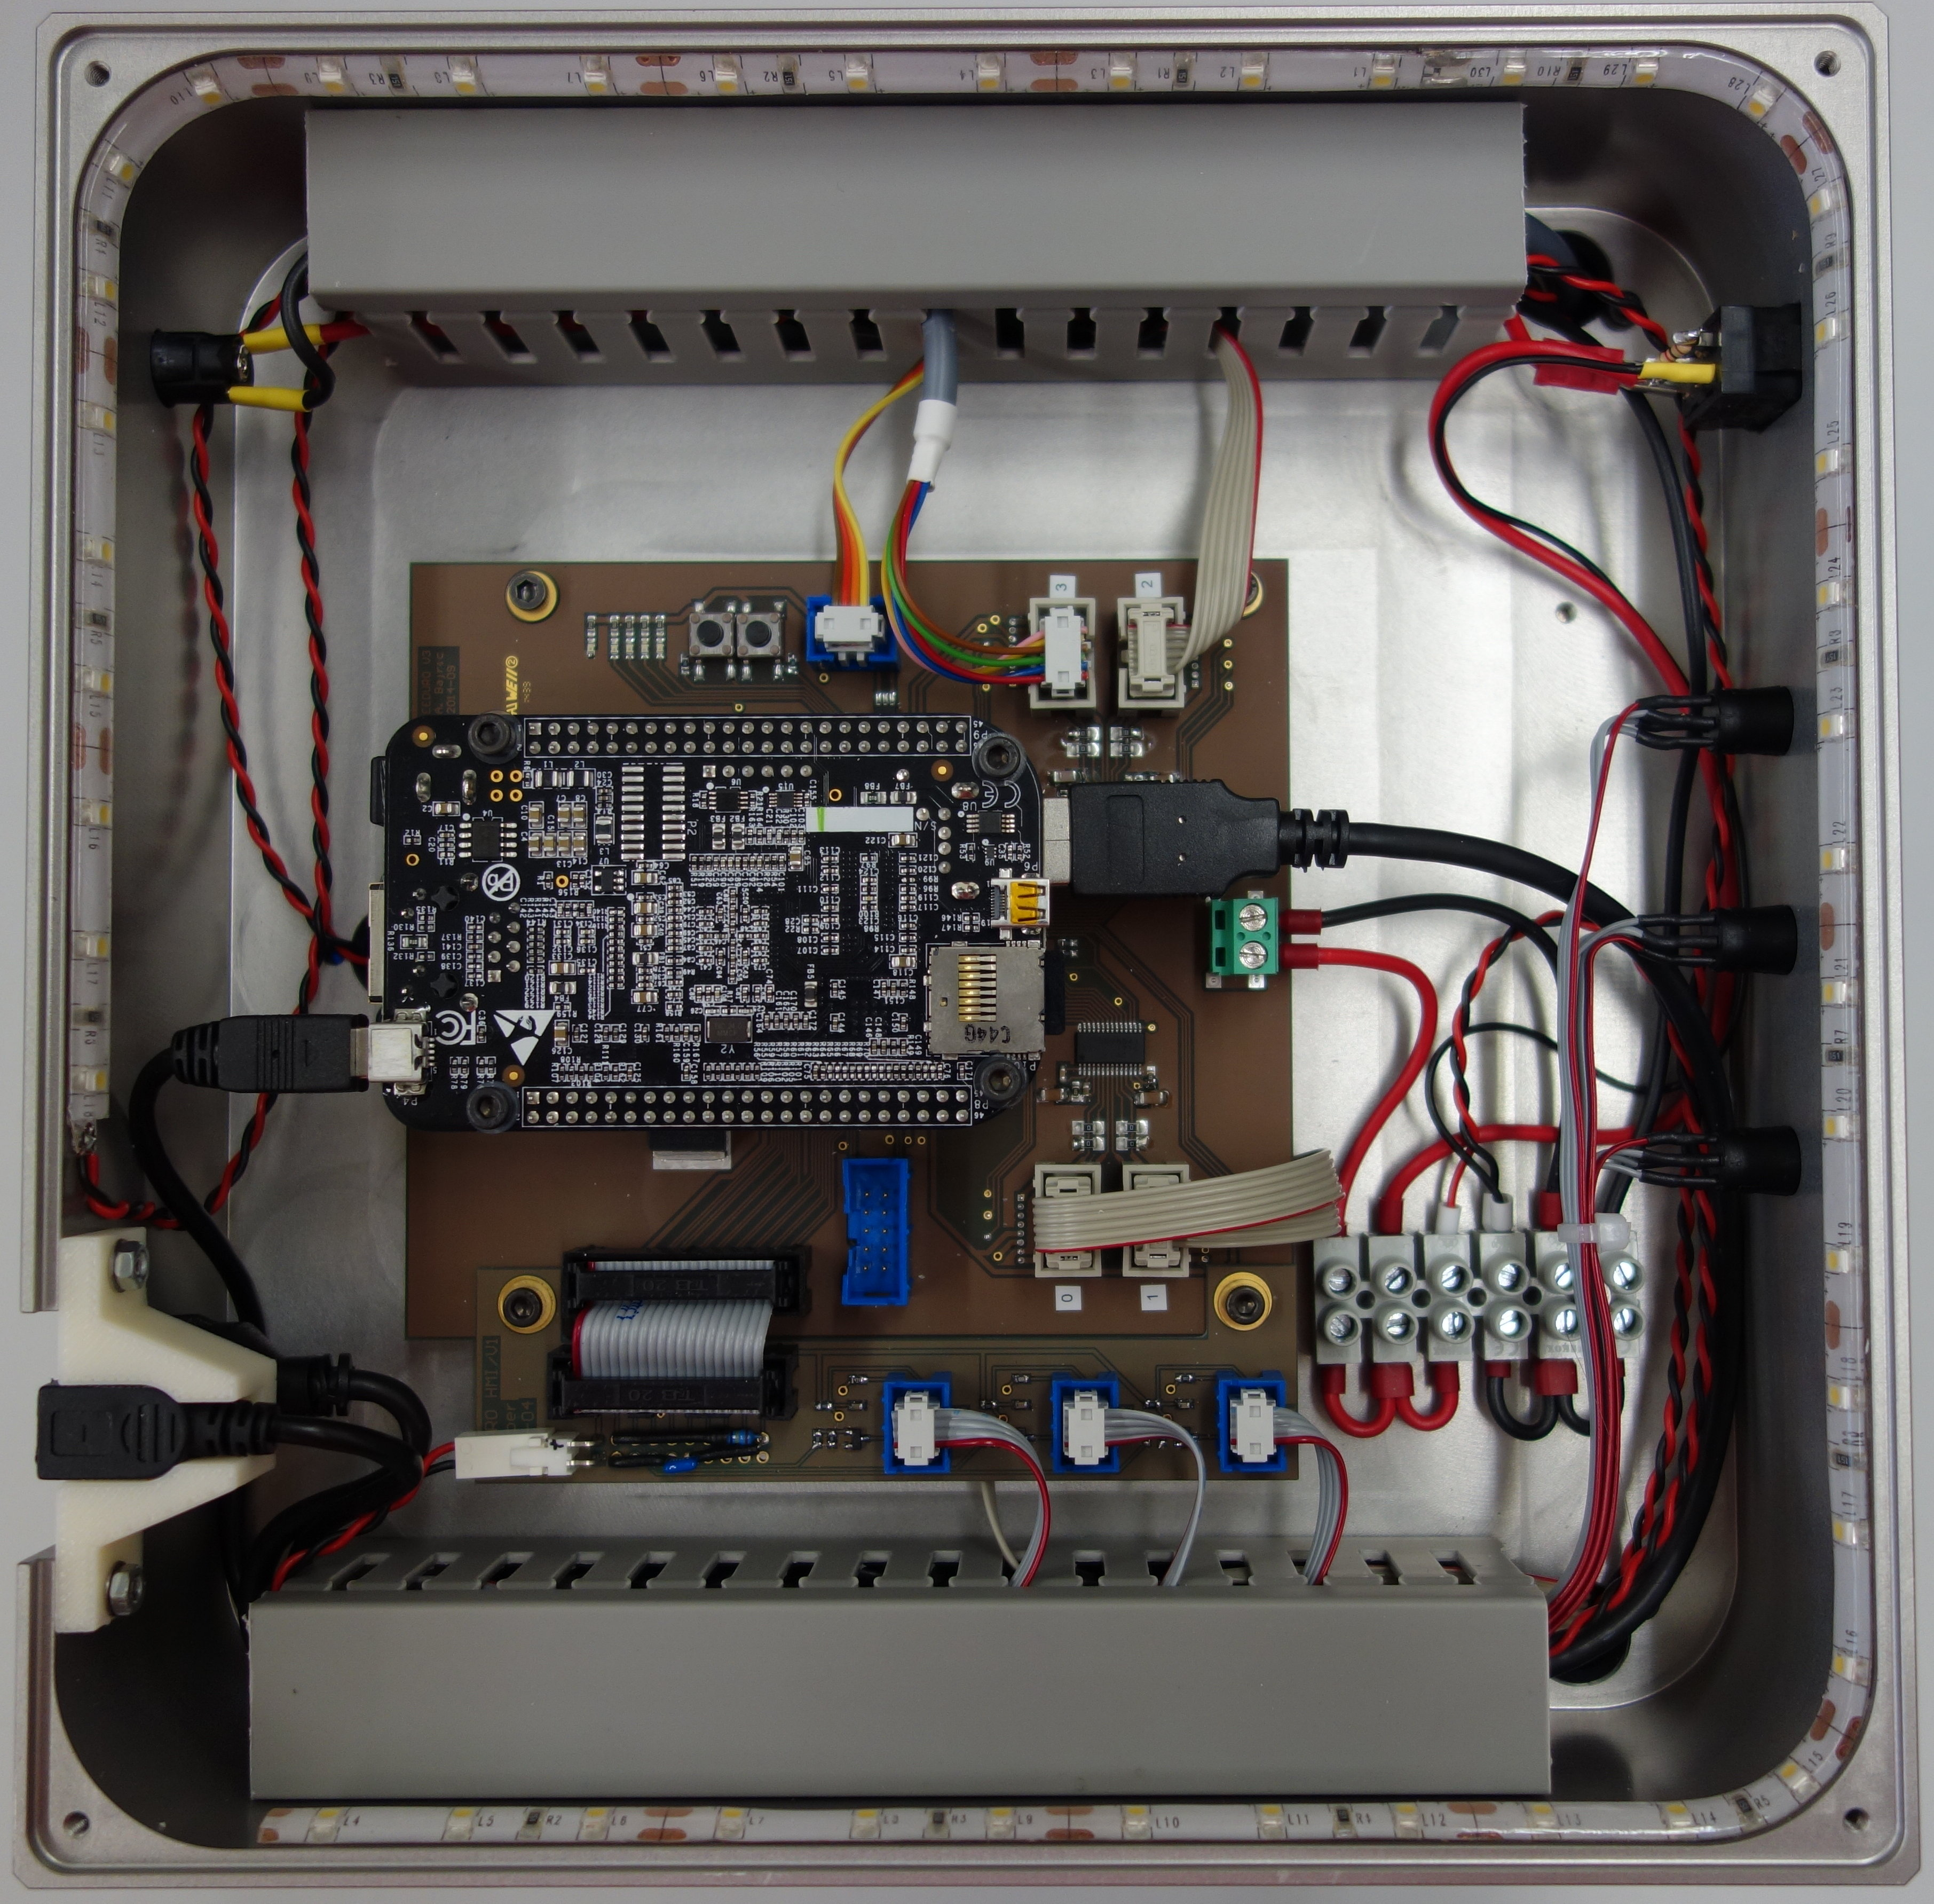
\includegraphics[width=0.7\textwidth]{BaseCaseOpenWithBBB}
	\caption{Base case with BeagleBone Black mounted}
	\label{fig:BaseCaseOpenWithBBB}
\end{figure}

\subsection{Mounting the BeagleBone in the remote case}
\begin{enumerate}
	\item Ensure that all cables are unplugged!
	\item Loose the four screws at the front of the case (see figure~\ref{fig:RemoteCaseFront}).
	\item Remove the front cover and the black plastic frame. Mind the cables for the buttons and the power switch when removing the cover!
	\item Draw out the closure head.
	\item Plug the BeagleBone on the headers in the middle of the main board as shown in figure~\ref{fig:RemoteCaseOpenWithBBB}.
	\item Fix the BeagleBone with four screws M3x10 (use polyamide washers).
	\item Plug the USB cable into the USB host connector (P3) on the BeagleBone.
	\item Insert the SD-Card shipped with the robot.
	\item Remount the closure head plate.
	\item Clip back the plastic frame and close the front cover.
	\item Fix the front cover with the four screws.
\end{enumerate}

\begin{figure}[htbp]
	\centering
	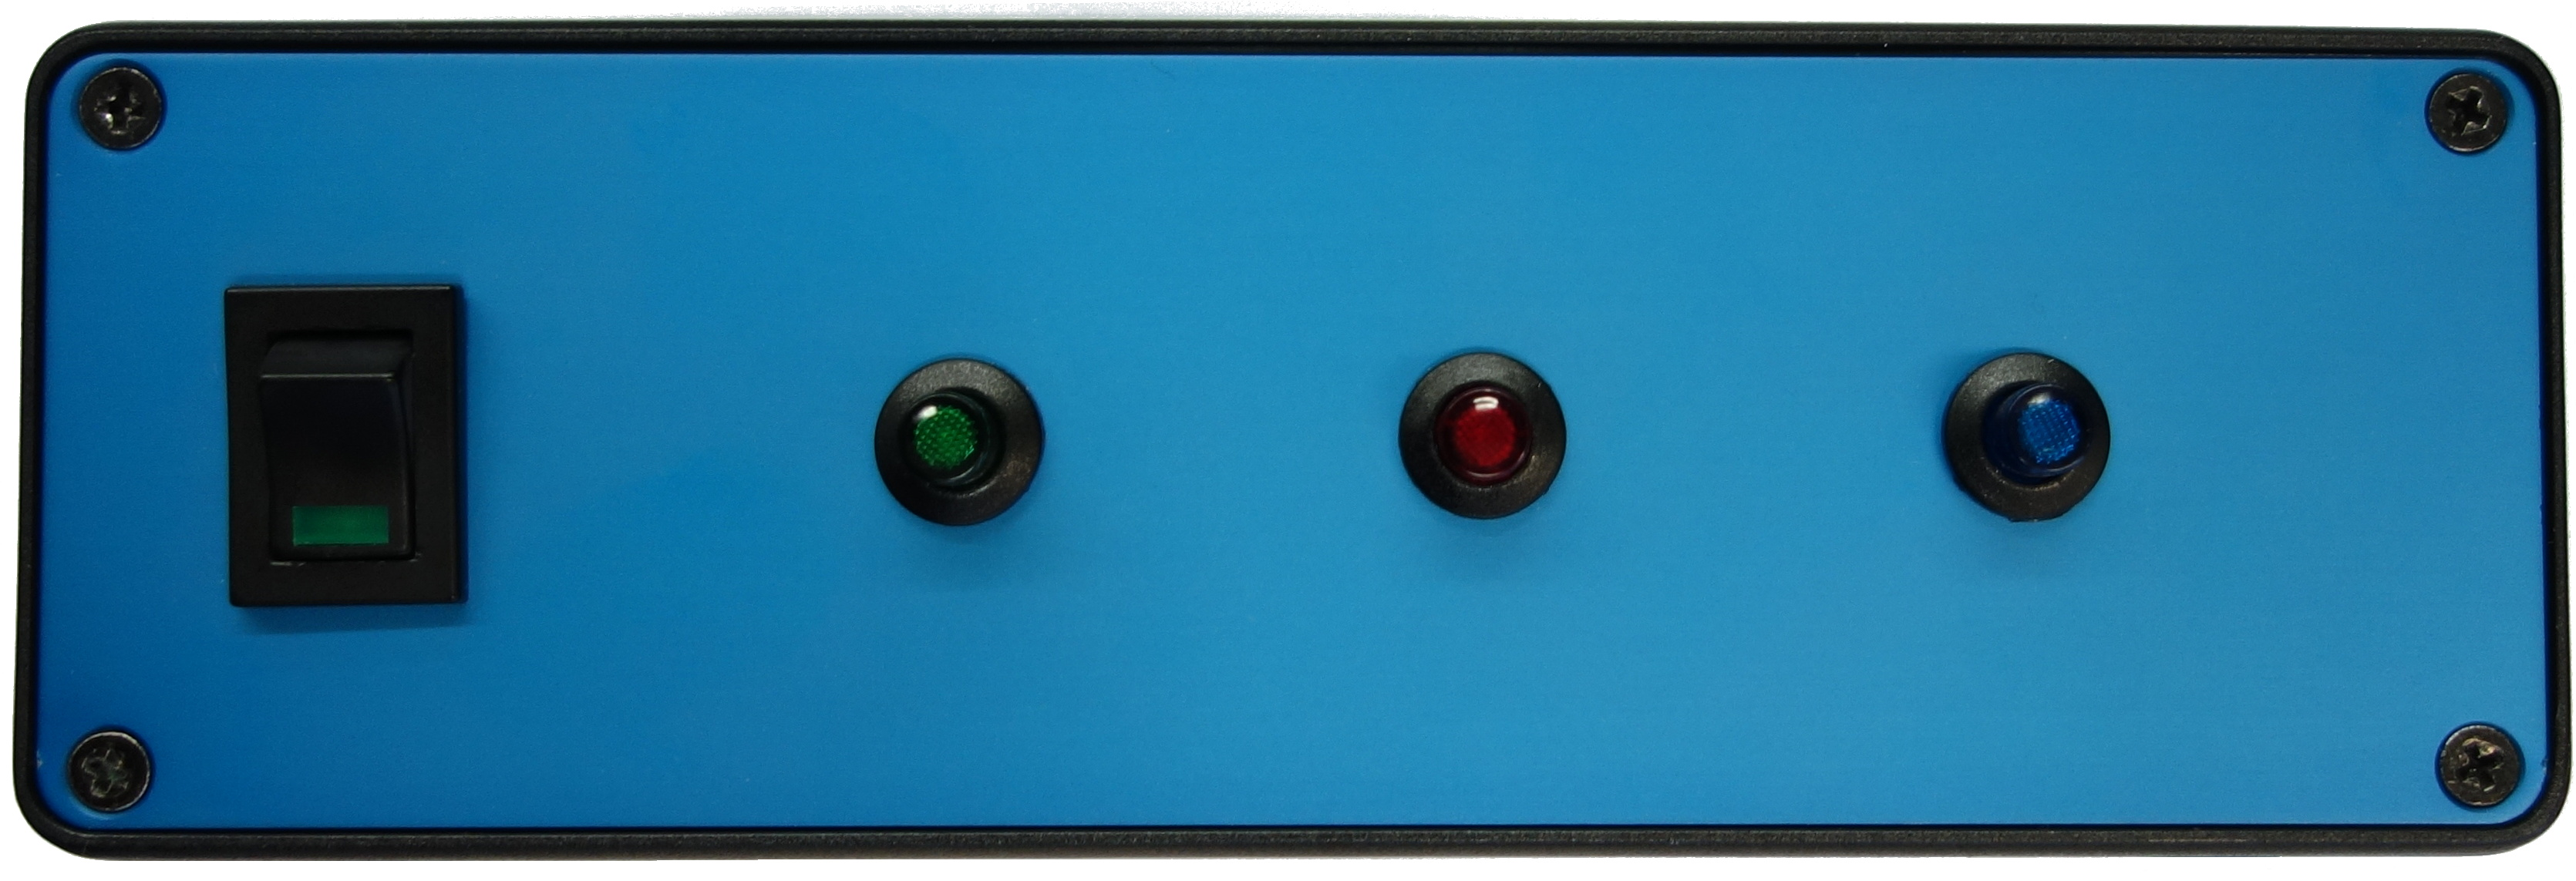
\includegraphics[width=\textwidth]{RemoteCaseFront}
	\caption{Remote case front view}
	\label{fig:RemoteCaseFront}
\end{figure}

\begin{figure}[htbp]
	\centering
	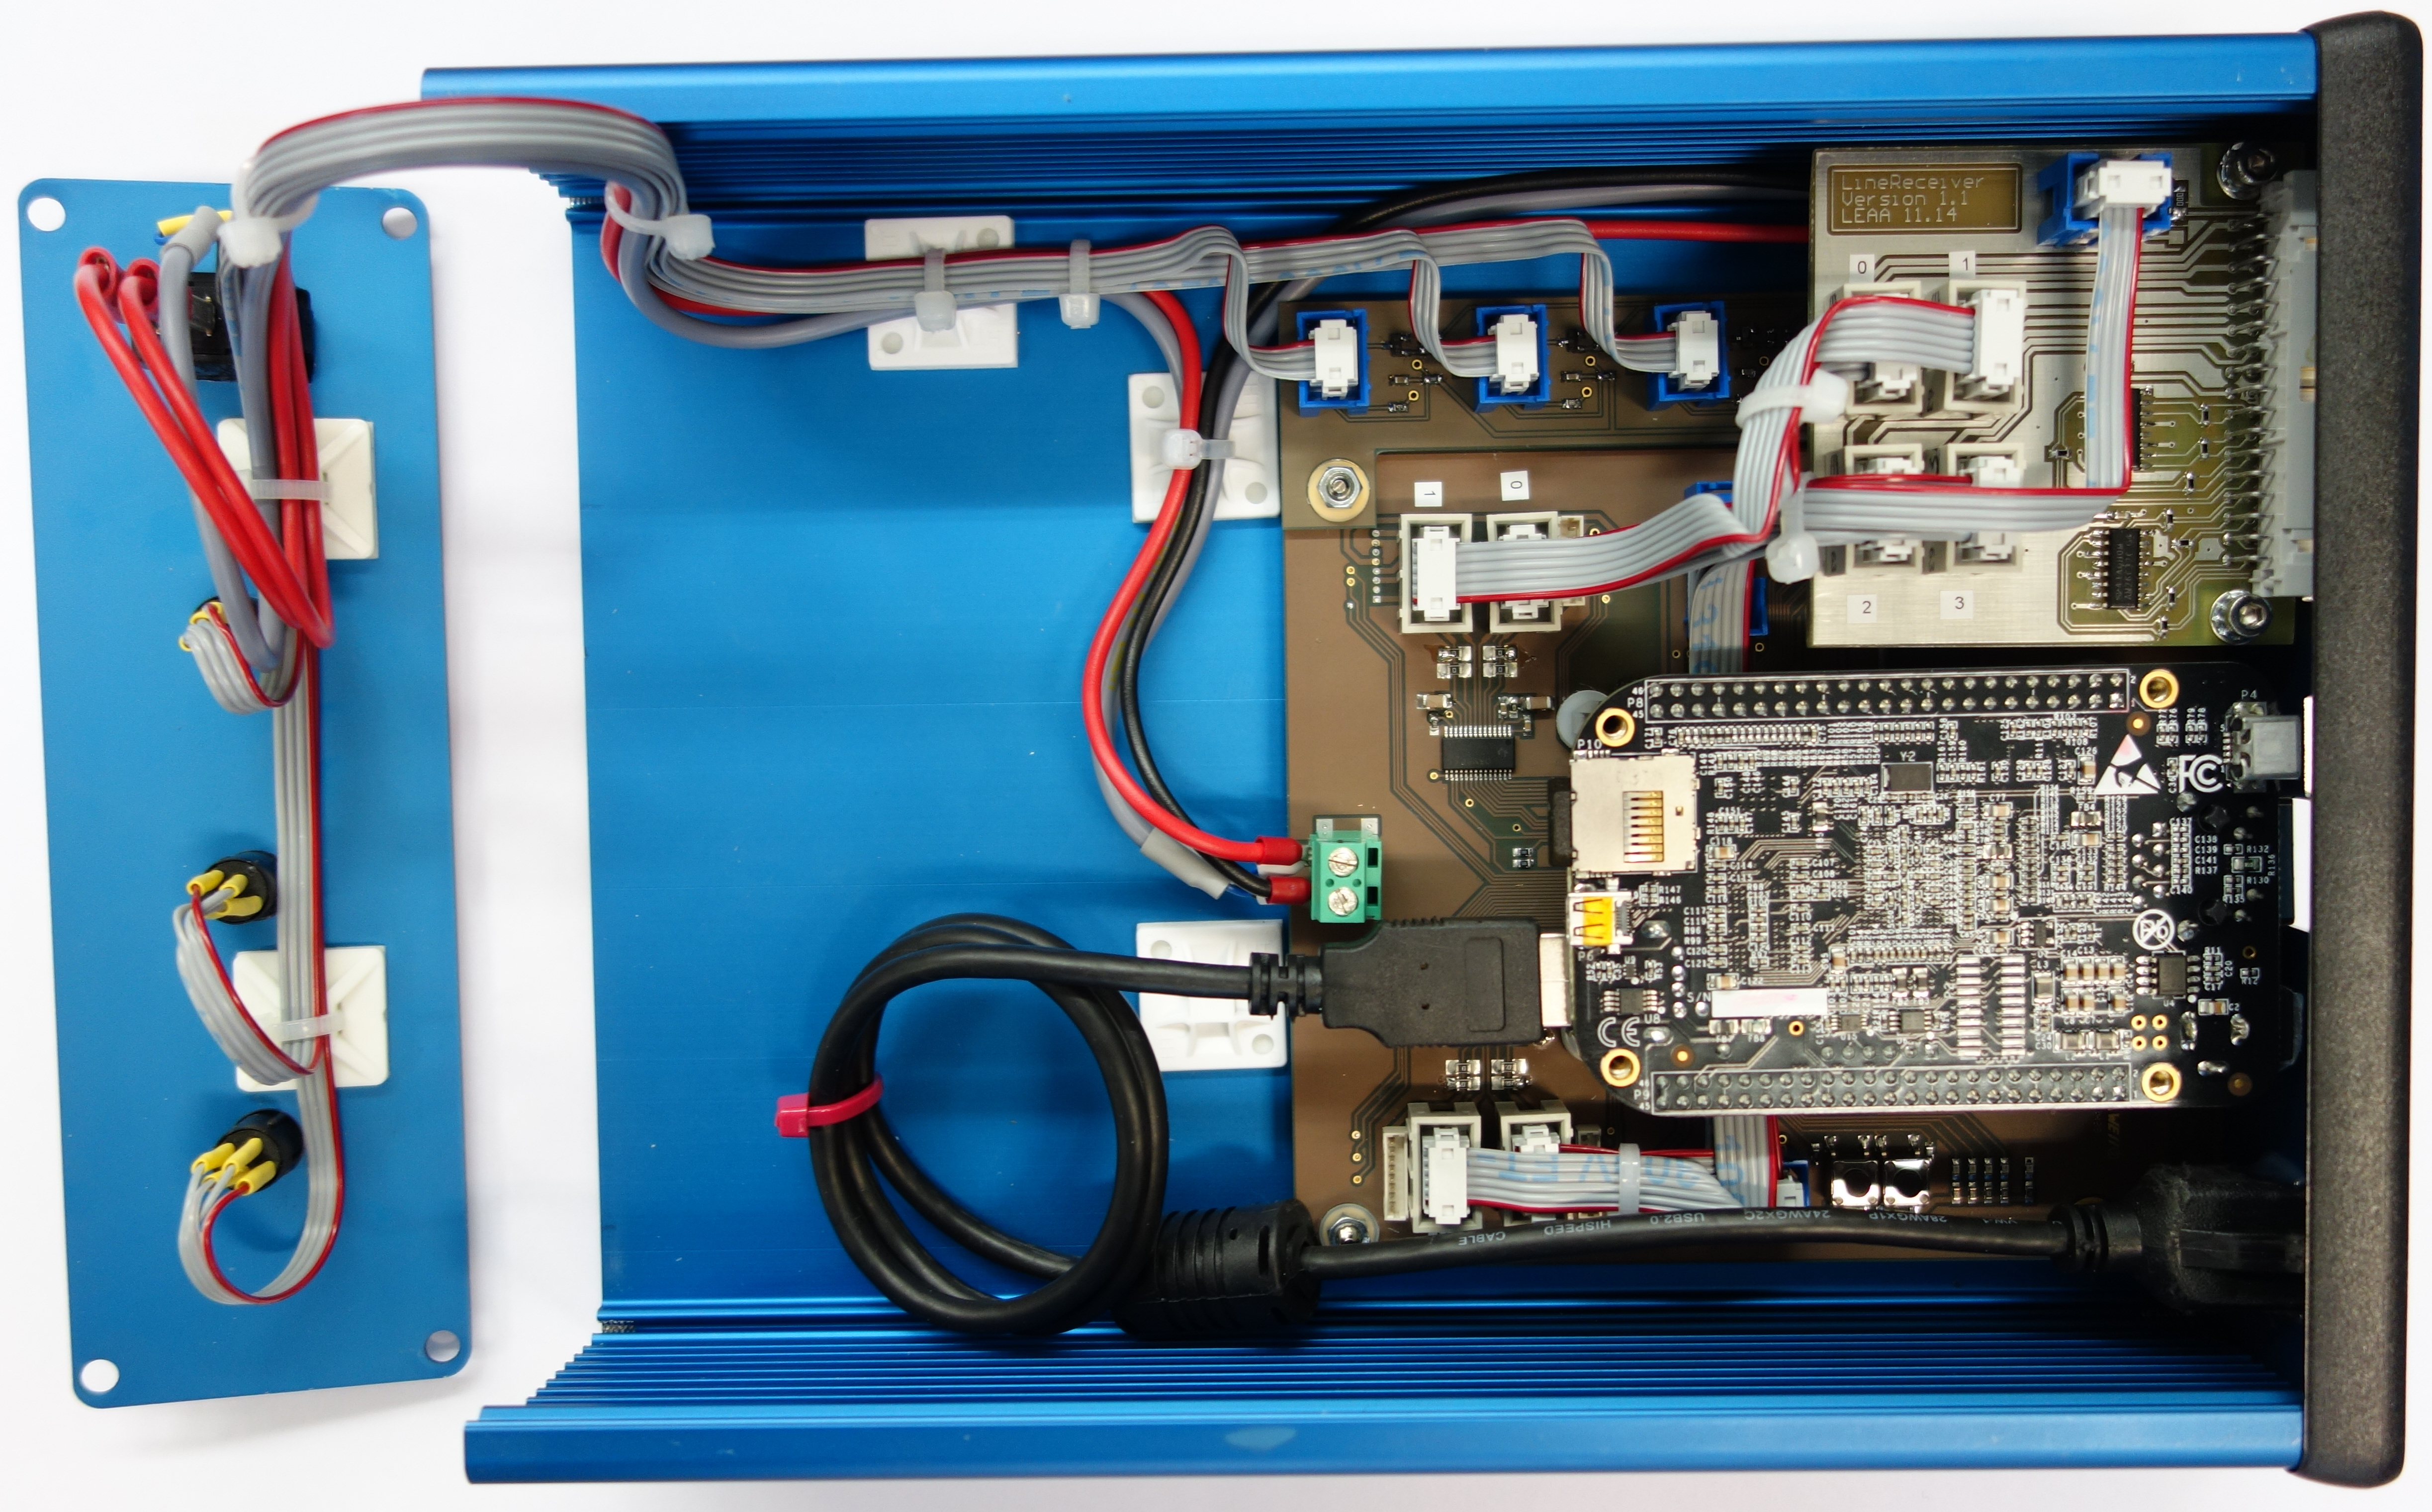
\includegraphics[width=\textwidth]{RemoteCaseOpenWithBBB}
	\caption{Remote case top view with BeagleBone Black mounted}
	\label{fig:RemoteCaseOpenWithBBB}
\end{figure}

\section{First start}
\begin{enumerate}
	\item Connect the power supply to the power connector X5 on the rear side. Use a power supply with 12\,VDC output and at least 1.5\,A. The coaxial power connector is a Type A according to IEC60130-10 with negative barrel.
	\item Connect a PC mouse and/or a Microsoft XBox remote controller to the USB Port X1.
	\item Switch on the robot using the power switch at the front.
	\item Wait until the green button at the front starts lighting.
	\item Ensure the working room of the robot is clear and press the green button. Caution: the robot now moves for initialization!
	\item After initialization is done, there are three demo applications available. The default application allows to control the TCP with the mouse. With the second application the TCP can be controlled by the XBox Controller. The third demo application moves the TCP to some predefined positions. You can choose an application by pressing the blue button.
\end{enumerate}

\chapter{Setup a development environment}
To develop software for the EEDURO platform, you will need a Linux based operating system. Any modern Linux distribution can be used.

\begin{enumerate}
	\item All required source code is hosted in a git repository at github.com. So the first step is to install the git client and all necessary build tools: git, g++ (version 4.7 or newer), CMake (version 2.8 or newer) and GNU Make. On a Debian based distribution you can install this by typing:
		\begin{verbatim}
		$ sudo apt-get install git g++ cmake make
		\end{verbatim}
	\item There are a handful of bash scripts available, which helps you setting up the develop environment. Clone the \texttt{eeduro-scripts} repository:
		\begin{verbatim}
		$ git clone git://github.com/eeros-project/eeduro-scripts.git eeduro-project
		\end{verbatim}
	\item Change into the \texttt{eeduro-project} folder and execute the \texttt{setup.sh} shell script.
		\begin{verbatim}
		$ cd eeduro-project
		$ ./setup.sh
		\end{verbatim}
		The setup script checks if all packages are installed, clones the \texttt{eeros-framework} repository, clones the \texttt{eeduro-platform repository}, downloads the Linaro toolchain and creates folders for local and cross builds.
	\item Now you can enter the \texttt{build-armhf} directory and build the software:
		\begin{verbatim}
		$ cd build-armhf
		$ make
		\end{verbatim}
	\item The copy2robot.sh shell script copies all the generated binaries to the robot. The script is configured to use the robot connected by USB. If you've connected the robot by ethernet, you have to adjust the script by setting the correct ip address of the robot.
\end{enumerate}


\chapter{Start programming}
TODO Adam

\end{document}
